% !TeX spellcheck = en_GB
\def\ChapterTitle{Assessment of \gls{tmf} Performance in Marine Environments}

\chapter{\ChapterTitle}
\label{Chapter\thechapter}
\lhead{Chapter \thechapter. \emph{\nameref{Chapter\thechapter}}} % Write in your own chapter title to set the page header


\section{Introduction}


As \glspl{manet} grow beyond the terrestrial arena, their operation and the protocols designed around them must be reviewed to assess their suitability to different communications environments to ensure their continued security, reliability, and performance.
With demand for smaller, more decentralised \gls{manet} systems in a range of domains and applications, as well as a drive towards lower per-unit cost in all areas, \glspl{tmf} are going to be increasingly applied to resource constrained applications, as the benefits and efficiencies they present are significant.
This work is primarily concerned with the analytical establishment of hard trust within a topologically dynamic network of autonomous actors.
Beyond the constraints of the communications environment, knock on pressures in battery capacity, on-board processing, and locomotion simultaneously present opportunities and incentives for malicious or selfish actors to appear to cooperate while not reciprocating, in order to conserve power for instance.
These multiple aspects of potential incentives, trust, and fairness do not directly fall under the scope of single metric trusts discussed above, and this context indicates that a multi-metric approach may be more appropriate.
These increasingly decentralised applications present unique threats against trust management \cite{Caiti2011}.

Previous research has established the advantages of implementing \glspl{tmf} in 802.11 based \glspl{manet}, particularly in terms of preventing selfish operation in collaborative systems \cite{Li2007}, and maintaining throughput in the presence of malicious actors \cite{Buchegger2002}

To date this work has been limited to terrestrial, RF based networks. 

One area of application is the underwater marine environment, where extreme challenges to communications present themselves (propagation delays, frequency dependent attenuation, fast and slow fading, refractive multipath distortion, etc.)(\autoref{Chapter3}).
In addition to the communications challenges, other considerations such as command and control isolation, as well as power and locomotive limitations, drive towards the use of teams of smaller and cheaper \gls{auv} platforms.
In underwater environments, communications is both sparse and noisy.
Therefore the observations about the communications processes that are used to generate the trust metrics, occur much less frequently, with much greater error (noise) and delay than is experienced in terrestrial RF \glspl{manet}.

In addition to the communications challenges, other considerations such as command and control isolation, as well as power and locomotive limitations, drive towards the use of teams of smaller and cheaper \glspl{auv}.
As such, the use of trust methods developed in the terrestrial \gls{manet} space must be re-appraised for application within the underwater context \cite{Pavan2015}.
Many \glspl{uan} use \gls{manet} architectures, however the marine environment presents new challenges for trust management frameworks that have been developed for use in conventional (i.e. Terrestrial RF) \glspl{manet}.

It is shown that single metric trust systems are not directly suitable for the marine context in terms of the different threat and cost scenario in that environment.

These single metric \glspl{tmf} provide malicious actors with a significant advantage if their activity does not impact that metric.
In the case where the attacker can subvert the \gls{tmf}, the metric under assessment by that \gls{tmf} does not cover the threat mounted by the attacker.
This causes a significant negative effect on the efficiency of the network, as the \gls{tmf} is assumed to have reduced the possible set of attacks when it has actually made it more advantageous to attack a different part of the networks operation.
An example of such a situation would be in a \gls{tmf} focused on \gls{plr} where an attacker selectively delays packets going through it, reducing overall throughput but not dropping any packets.
Such behaviour would not be detected by the \gls{tmf}.

For the purposes of this work, from those \glspl{tmf} discussed in~\autoref{sec:c2_tmfs}, Hermes trust establishment, \gls{otmf} and \gls{mtfm} are selected as indicative single and multi metrics frameworks for comparison, as Hermes captures the core operation of a pure single metric assessment methodology and \gls{otmf} provides a comparison that combines assessments from across nodes to develop trust opinions.

From the discussion on the nature of the communications environment in~\autoref{sec:trust_in_marine}, it's clear that before assessing communications metrics a simulated underwater environment, appropriate scaling factors must be found that are realistic from an application perspective but are also comperable in some form to the \gls{manet} case.


\section{Modelling of \gls{uan} network}\label{sec:initialsystemcharacterization}


\subsection{Mobility, Topology, and Communications}

Four mobility patterns are investigated:
\begin{enumerate}
	\item All Nodes Static
	\item Malicious node mobile
	\item Malicious node mobile, all other nodes static
	\item All nodes mobile
\end{enumerate}

For this case, the mobility model used is a random walk on the nodes modeled kinematic response, i.e.\ the node periodically picks a spherically normalised random direction in the XY plane.
Maximum node speed (limited by kinematic acceleration/turning constraints) is 1.5$ms^{-1}$.


The six nodes are initially arranged as per Fig.~\ref{fig:s1_layout} with each node on average 100m from each other as per \cite{Guo11}.
The use of six nodes and the particular layout enables the investigation of the three trust relationships based on minimum path topologies, such that the node generating the trust assessments, $n_0$ has Direct, Recommendation, and Indirect trust assessments of $n_1$ available to it from itself, $[n_2,n_3]$, and $[n_4,n_5]$ respectively. 
(See Section~\ref{sec:trust_topologies})

Collaborations with NATO \gls{cmre} in La Spezia, and \glspl{dstl} Naval Systems Group inform that this is a practical team-size for environmental and defence applications.

%
\begin{figure}[h]
	\centering
	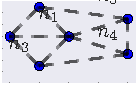
\includegraphics[width=.45\textwidth]{s1_layout}
	\caption{Initial layout with nodes spaced an average of 100m apart}
	\label{fig:s1_layout}
\end{figure}
%

\subsection{Simulation Background}

Simulations were conducted using a Python based simulation framework, SimPy \cite{Mueller2003SimPy}, with a network stack built upon AUVNetSim \cite{Miquel2008}, with transmission parameters (\autoref{tab:sysconstraints}) taken from and validated against \cite{Stojanovic2007}, \cite{Stefanov2011} and \cite{Sehgal2010}\todo{it would be worth while going through this verification explicitly as an appendix}

Given the differences in delay and propagation between RF and marine networks, it would not be expected that the same application rates (e.g.\ packet emission rates or throughput) and node separations are equally stable in this environment.
Therefore, a zone of performance is characterised within which the network has stable operation.
%
\begin{table}[h]
	\caption{Comparison of system model constraints as applied between Terrestrial and Marine communications} \label{tab:sysconstraints}
	\begin{center}
		\setlength{\tabcolsep}{8pt}
		\begin{tabular}{lccc}
			\toprule
			Parameter & Unit & Terrestrial & Marine \\
			\midrule
			Simulated Duration & $s$ & 300 & 18000\\
			Trust Sampling Period & $s$ & 1 & 600 \\
			Simulated Area & $km^2$ & 0.7 & 0.7-4 \\
			Transmission Range & $km$ & 0.25 & 1.5 \\
			Physical Layer & & RF(802.11) & Acoustic\\
			Propagation Speed& $m/s$ & $3\times10^8$ & 1490\\
			Center Frequency& $Hz$ & $2.6\times10^9$ & $2 \times 10^4$ \\
			Bandwidth& $Hz$ & $22\times10^6$ & $1\times10^4$\\
			MAC Type & & CSMA/DCF & CSMA/CA\\
			Routing Protocol & & DSDV & FBR \\
			Max Speed & $ms^{-1}$ & 5 & 1.5 \\
			Max Data Rate & $bps$ & $5\times10^6$ & $\approx 240$ \\
			Packet Size & bits & 4096 &  9600 \\
			Single Transmission Duration & $s$ & 10 & 32 \\
			Single Transmission Size & bits & $10^7$ & $9600$ \\
			\bottomrule
		\end{tabular}
		\setlength{\tabcolsep}{6pt}
	\end{center}
\end{table}
%


\section{Establishing Scale Factors in Communications Rate}

In this section the simulated communications environment is characterised to establish an optimal packet emission rate for comparison against \cite{Guo11}.
This optimal emission rate is taken to be an emission rate that provides reasonable network stability and protection from network saturation.
Network saturation is the point at which a network can no longer successfully deliver the offered load\footnote{It will become important to note that Offered Load in this case includes packet retransmissions} presented to it to the relevant destinations (throughput), and is characterised by a peak and a subsequent decline in the throughput of the network when varying the packet emission rate. 

In order to establish the point at which the network becomes saturated due, a range of packet emission rates were explored between 0.01 packets per second (pps), equivalent to 96 bits of offered load per node, up to 0.07 pps (672 bps per node).
Initial node separation was set as per Guo at 100$m$, and each simulation is run 16 times, with each instance modelling a 8 hour mission time.\todo[inline]{Need to have a discussion about mission configurations at some point}

Looking first at the Static mobility case, where all nodes are stationary; from~\autoref{fig:emission_throughput_performance_bella_static} it is already clear that the throughput curve, exhibits a saturation point close to 0.025 pps.
Similarly in~\autoref{fig:emission_prod_breakdown_bella_static}, the precipitous drop in packet delivery probability beyond 0.025 pps, indicating that this is a strong candidate value for an upper-limit to the safe operating zone in terms of packet emission in the small static case.
From~\autoref{fig:emission_delay_variation_bella_static}, raising packet emissions above 0.25pps results in a significant increase in end-to-end delay.
As per~\autoref{tab:sysconstraints}, the CSMA based \gls{mac} incurs a certain amount of control overhead in the form of \gls{rts} packets, when a node attempts to acquire time in its neighbourhood.
In~\autoref{fig:emission_rts_ratio_bella_static}, the ratio of Control/Data packets increases linearly up to 1.5 until just before 0.025pps, and then accelerates to almost 2.5, further demonstrating that the network has become critically congested.
It is worthwhile noting that in~\autoref{fig:emission_throughput_performance_bella_static} that even as the saturation point is passed, packet collisions do not significantly increase, and that the saturation is in fact driven by contention in the medium rather than congestion-collisions.

Results are also included from the remaining mobility cases (all nodes mobile; all-but-one node mobile; single mobile node), however from Figs.~\ref{fig:emission_all},~ \ref{fig:emission_bella_all_mobile}-~\ref{fig:emission_bella_single_mobile} that the throughput threshold behaviour is qualatitively similar regardless of mobility for this initial node separation.


\begin{figure}[h]
  \begin{subfigure}[t]{0.5\textwidth}
    \centering
    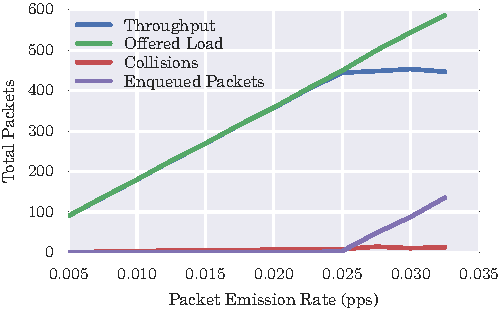
\includegraphics[width=\textwidth]{emission_throughput_performance_bella_static}
    \caption{Static}
    \label{fig:emission_throughput_performance_sum_bella_static}
  \end{subfigure}
  \begin{subfigure}[t]{0.5\textwidth}
    \centering
    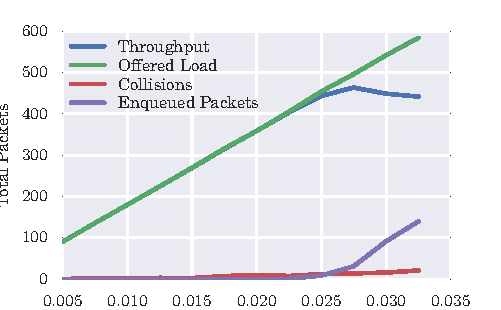
\includegraphics[width=\textwidth]{emission_throughput_performance_bella_all_mobile}
    \caption{All Mobile}
    \label{fig:emission_throughput_performance_sum_bella_all_mobile}
  \end{subfigure}  
  
  \begin{subfigure}[t]{0.5\textwidth}
    \centering
    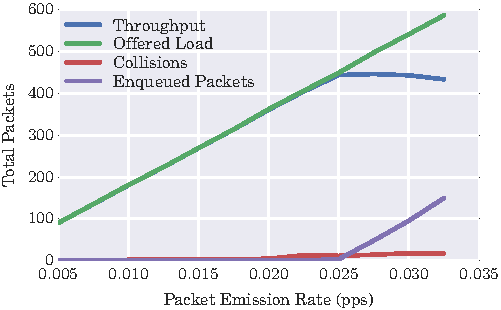
\includegraphics[width=\textwidth]{emission_throughput_performance_bella_allbut1_mobile}
    \caption{All-but-one Mobile}
    \label{fig:emission_throughput_performance_sum_bella_allbut1_mobile}
  \end{subfigure}  
  \begin{subfigure}[t]{0.5\textwidth}
    \centering
    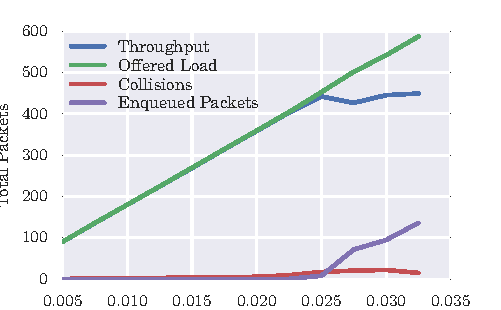
\includegraphics[width=\textwidth]{emission_throughput_performance_bella_single_mobile}
    \caption{Single Mobile}
    \label{fig:emission_throughput_performance_sum_bella_single_mobile}
  \end{subfigure}
  \caption{Throughput performance overview for all mobilities under varying emission rates\emph{IS THIS ENOUGH?}}
  \label{fig:emission_all}
\end{figure}


\begin{figure}[tp!]
  \begin{subfigure}[t]{0.5\textwidth}
    \centering
    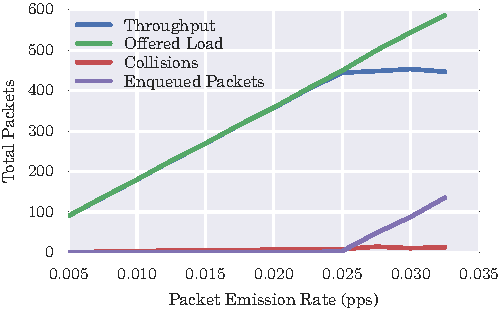
\includegraphics[width=\textwidth]{emission_throughput_performance_bella_static}
    \caption{Packet delivery}
    \label{fig:emission_throughput_performance_bella_static}
  \end{subfigure}
  %
  \begin{subfigure}[t]{0.5\textwidth}
    \centering
    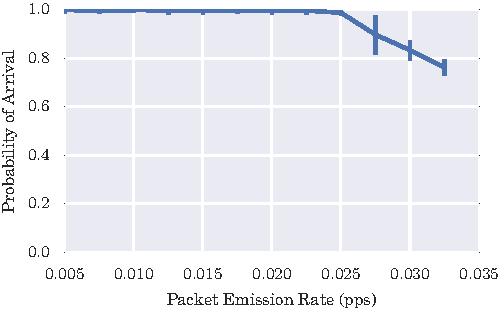
\includegraphics[width=\textwidth]{emission_prod_breakdown_bella_static}
    \caption{Probability of arrival}
    \label{fig:emission_prod_breakdown_bella_static}
  \end{subfigure}

  \begin{subfigure}[t]{0.5\textwidth}
    \centering
    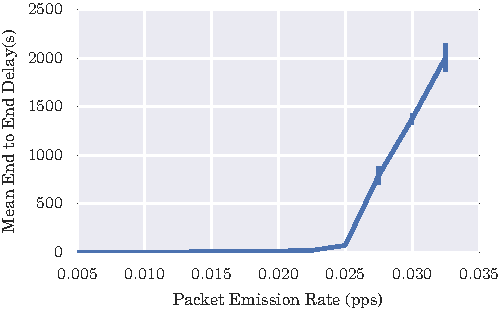
\includegraphics[width=\textwidth]{emission_delay_variation_bella_static}
    \caption{End-to-end delay}
    \label{fig:emission_delay_variation_bella_static}
  \end{subfigure}
  %
  \begin{subfigure}[t]{0.5\textwidth}
    \centering
    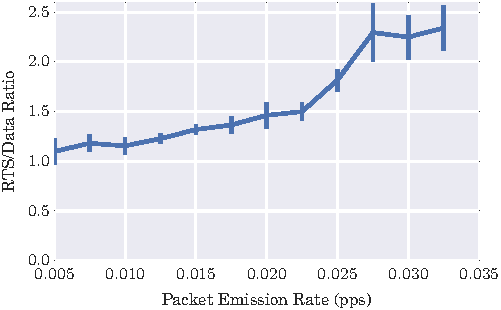
\includegraphics[width=\textwidth]{emission_rts_ratio_bella_static}
    \caption{RTS Ratios}
    \label{fig:emission_rts_ratio_bella_static}
  \end{subfigure}
  \caption{Network performance varying packet emission rates for the static case}
  \label{fig:emission_bella_static}
\end{figure}


\begin{figure}[bp!]
  \begin{subfigure}[t]{0.5\textwidth}
    \centering
    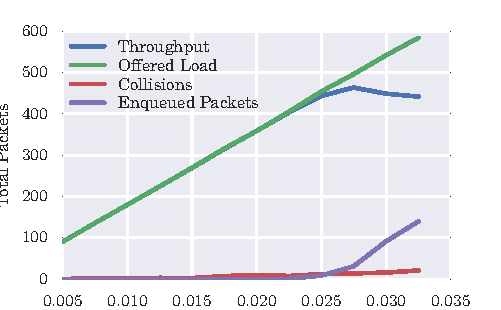
\includegraphics[width=\textwidth]{emission_throughput_performance_bella_all_mobile}
    \caption{Packet delivery}
    \label{fig:emission_throughput_performance_bella_all_mobile}
  \end{subfigure}
  %
  \begin{subfigure}[t]{0.5\textwidth}
    \centering
    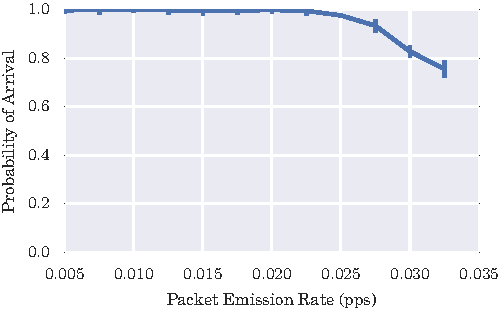
\includegraphics[width=\textwidth]{emission_prod_breakdown_bella_all_mobile}
    \caption{Probability of arrival}
    \label{fig:emission_prod_breakdown_bella_all_mobile}
  \end{subfigure}

  \begin{subfigure}[t]{0.5\textwidth}
    \centering
    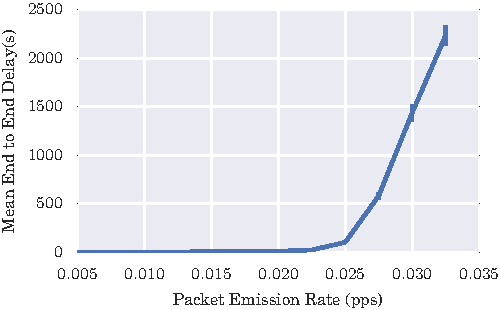
\includegraphics[width=\textwidth]{emission_delay_variation_bella_all_mobile}
    \caption{End-to-end delay}
    \label{fig:emission_delay_variation_bella_all_mobile}
  \end{subfigure}
  %
  \begin{subfigure}[t]{0.5\textwidth}
    \centering
    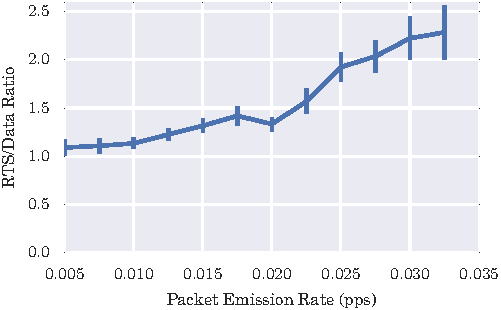
\includegraphics[width=\textwidth]{emission_rts_ratio_bella_all_mobile}
    \caption{RTS Ratios}
    \label{fig:emission_rts_ratio_bella_all_mobile}
  \end{subfigure}
  \caption{Network performance varying packet emission rates for the all mobile case}
  \label{fig:emission_bella_all_mobile}
\end{figure}


\begin{figure}[tp!]
  \begin{subfigure}[t]{0.5\textwidth}
    \centering
    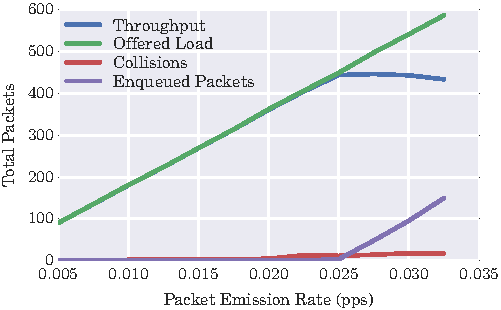
\includegraphics[width=\textwidth]{emission_throughput_performance_bella_allbut1_mobile}
    \caption{Packet delivery}
    \label{fig:emission_throughput_performance_bella_allbut1_mobile}
  \end{subfigure}
  %
  \begin{subfigure}[t]{0.5\textwidth}
    \centering
    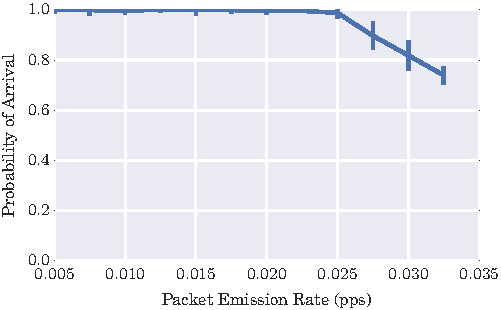
\includegraphics[width=\textwidth]{emission_prod_breakdown_bella_allbut1_mobile}
    \caption{Probability of arrival}
    \label{fig:emission_prod_breakdown_bella_allbut1_mobile}
  \end{subfigure}

  \begin{subfigure}[t]{0.5\textwidth}
    \centering
    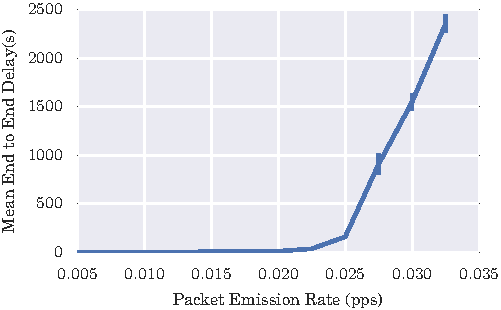
\includegraphics[width=\textwidth]{emission_delay_variation_bella_allbut1_mobile}
    \caption{End-to-end delay}
    \label{fig:emission_delay_variation_bella_allbut1_mobile}
  \end{subfigure}
  %
  \begin{subfigure}[t]{0.5\textwidth}
    \centering
    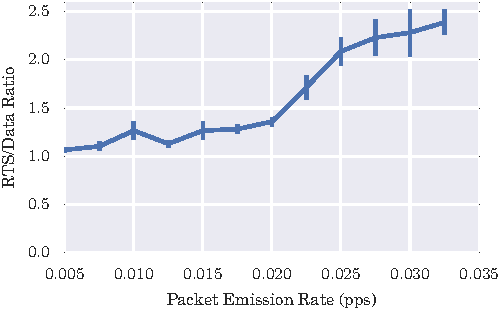
\includegraphics[width=\textwidth]{emission_rts_ratio_bella_allbut1_mobile}
    \caption{RTS Ratios}
    \label{fig:emission_rts_ratio_bella_allbut1_mobile}
  \end{subfigure}
  \caption{Network performance varying packet emission rates for the all-but-one mobile case}
  \label{fig:emission_bella_allbut1_mobile}
\end{figure}

\begin{figure}[bp!]
  \begin{subfigure}[t]{0.5\textwidth}
    \centering
    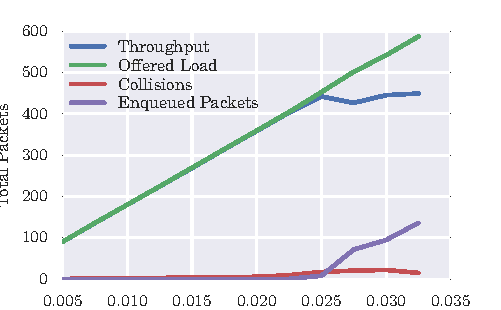
\includegraphics[width=\textwidth]{emission_throughput_performance_bella_single_mobile}
    \caption{Packet delivery}
    \label{fig:emission_throughput_performance_bella_single_mobile}
  \end{subfigure}
  %
  \begin{subfigure}[t]{0.5\textwidth}
    \centering
    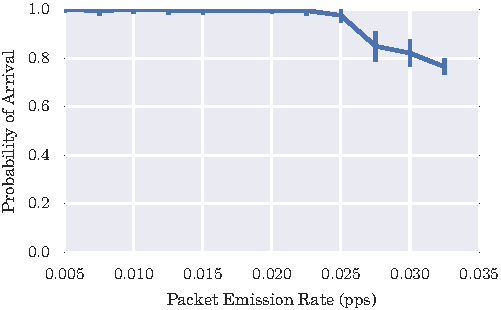
\includegraphics[width=\textwidth]{emission_prod_breakdown_bella_single_mobile}
    \caption{Probability of arrival}
    \label{fig:emission_prod_breakdown_bella_single_mobile}
  \end{subfigure}

  \begin{subfigure}[t]{0.5\textwidth}
    \centering
    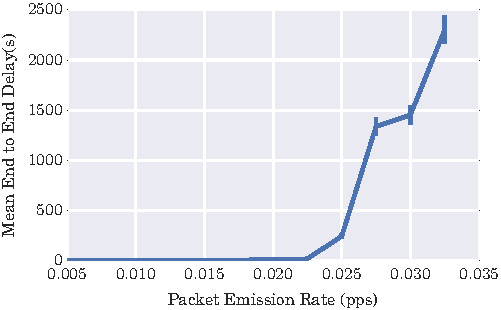
\includegraphics[width=\textwidth]{emission_delay_variation_bella_single_mobile}
    \caption{End-to-end delay}
    \label{fig:emission_delay_variation_bella_single_mobile}
  \end{subfigure}
  %
  \begin{subfigure}[t]{0.5\textwidth}
    \centering
    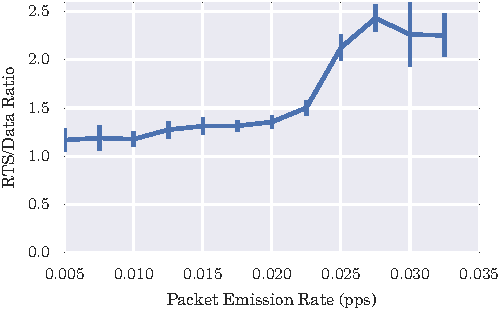
\includegraphics[width=\textwidth]{emission_rts_ratio_bella_single_mobile}
    \caption{RTS Ratios}
    \label{fig:emission_rts_ratio_bella_single_mobile}
  \end{subfigure}
  \caption{Network performance varying packet emission rates for the all-but-one mobile case}
  \label{fig:emission_bella_single_mobile}
\end{figure}

\clearpage

\subsection{Scale Factors in Physical Node Distribution}

In this section the effect of node-separation scaling on communications operation is characterised for comparison against \cite{Guo11}. 
This is particularly important considering the significant scale factor differences in terms of the speed of propagation in the medium, and the range of potential desired operation.

From~\autoref{tab:sysconstraints}, the operating transmission range of acoustic is $\approx 6$ times further than 802.11, indicating that a suitable operating environment will have an area $\approx \sqrt{6}$ times the area of the 802.11 case. Therefore, a reasonable experimental range would have an upper bound of performance around this scaling factor, where nodes are approximately 400$m$ apart. 

According to Xu, RTS/CTS handshake functionality cannot operate well as interference protection at node separations beyond 0.56 times the transmission range \cite{Xu2002}.
In the case of marine acoustic transmission at the stated power output, above $1500m \times 0.56 = 840m$, handshake overheads should begin to dominate channel access.\todo{redo these graphs with wider separations ~ 1000m}
This is due to reduced channel availability due to collisions, which are then due to a much longer potential contention period between nodes. 

A reasonable range around this is to scale from 100$m$ apart on average to 800$m$, and from the previous section, a packet emission rate of 0.02pps (slightly below the 0.025pps saturation threshold) is used to explore this space.

In the case where all nodes remain static, increasing node separation does not significantly impact throughput, delay, delivery probability or \gls{rts} ratios until rising above 700$m$ (Fig.~\ref{fig:separation_bella_static}), nearly double our initial estimate of where an appropriate separation zone would be.

The other mobility cases tell a very different story; as can be seen in~\autoref{fig:separation_throughput_performance_sum_bella_single_mobile}, where adding a single mobile node to the network induces a saturation-style response at 500$m$, and this drops further in~\autoref{fig:separation_throughput_performance_sum_bella_allbut1_mobile} and~\autoref{fig:separation_throughput_performance_sum_bella_all_mobile}, reducing the separation of saturation at this emission rate to just 300$m$.

Another aspect of these results to highlight is that the Offered Load presented to the network \emph{increases} beyond the collapse of the throughput curve. 
This indicates that there is a subtly different saturation behaviour with respect to separation than the simple congestion argument with respect to packet emission rate; packets are simply taking too long to cross the increasingly sparse network and in-transit packet routes are logically disconnected and require retransmission.
\todo[inline]{Another interesting aspect is the behaviour of the Enqueued Packet lines and e2e delay lines; They ``Bump''; no idea why yet}

\begin{figure}[h]
  \begin{subfigure}[t]{0.5\textwidth}
    \centering
    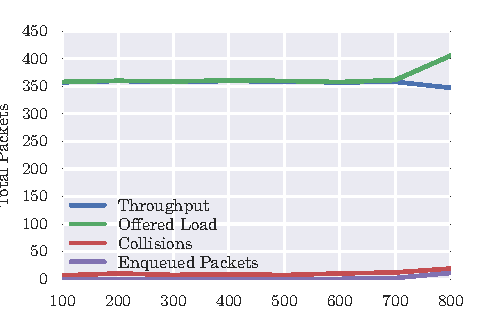
\includegraphics[width=\textwidth]{separation_throughput_performance_bella_static}
    \caption{Static}
    \label{fig:separation_throughput_performance_sum_bella_static}
  \end{subfigure}
  \begin{subfigure}[t]{0.5\textwidth}
    \centering
    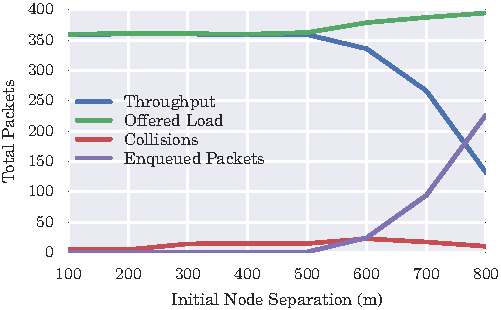
\includegraphics[width=\textwidth]{separation_throughput_performance_bella_single_mobile}
    \caption{Single Mobile}
    \label{fig:separation_throughput_performance_sum_bella_single_mobile}
  \end{subfigure}

  \begin{subfigure}[t]{0.5\textwidth}
    \centering
    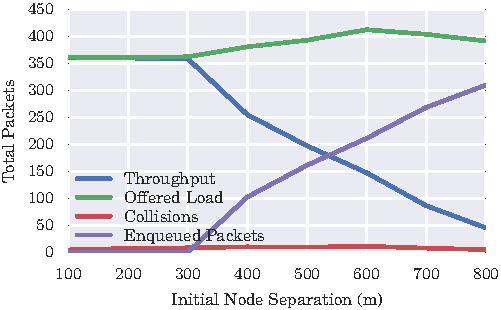
\includegraphics[width=\textwidth]{separation_throughput_performance_bella_allbut1_mobile}
    \caption{All-but-one Mobile}
    \label{fig:separation_throughput_performance_sum_bella_allbut1_mobile}
  \end{subfigure}  
  \begin{subfigure}[t]{0.5\textwidth}
    \centering
    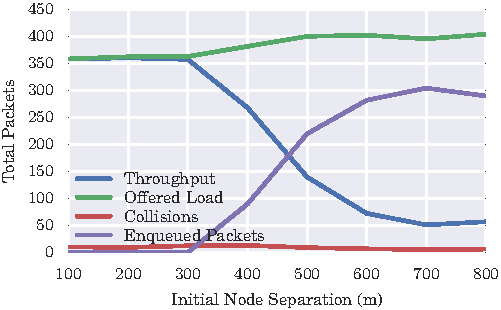
\includegraphics[width=\textwidth]{separation_throughput_performance_bella_all_mobile}
    \caption{All Mobile}
    \label{fig:separation_throughput_performance_sum_bella_all_mobile}
  \end{subfigure}  
  \caption{Throughput performance overview for all mobilities under varying separation \emph{IS THIS ENOUGH?}}
  \label{fig:separation_all}
\end{figure}

% These figures should be colocated
\begin{figure}[tp!]
  \begin{subfigure}[t]{0.5\textwidth}
    \centering
    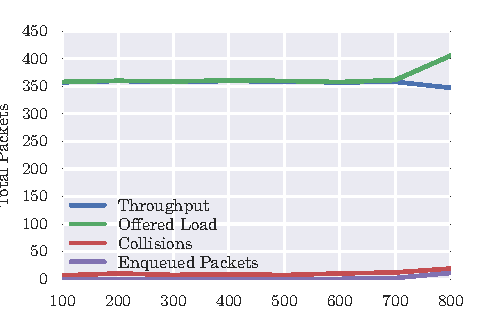
\includegraphics[width=\textwidth]{separation_throughput_performance_bella_static}
    \caption{Packet delivery}
    \label{fig:separation_throughput_performance_bella_static}
  \end{subfigure}
  %
  \begin{subfigure}[t]{0.5\textwidth}
    \centering
    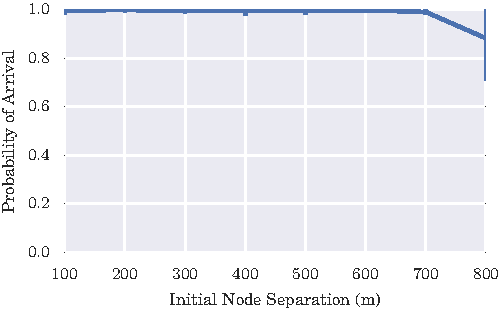
\includegraphics[width=\textwidth]{separation_prod_breakdown_bella_static}
    \caption{Probability of arrival}
    \label{fig:separation_prod_breakdown_bella_static}
  \end{subfigure}

  \begin{subfigure}[t]{0.5\textwidth}
    \centering
    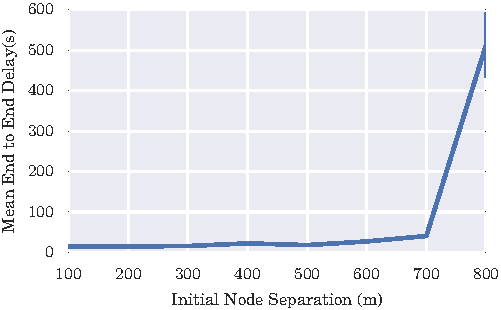
\includegraphics[width=\textwidth]{separation_delay_variation_bella_static}
    \caption{End-to-end delay}
    \label{fig:separation_delay_variation_bella_static}
  \end{subfigure}
  %
  \begin{subfigure}[t]{0.5\textwidth}
    \centering
    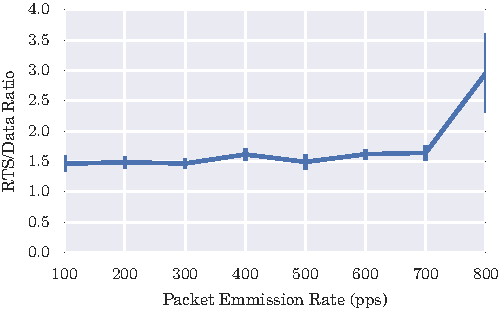
\includegraphics[width=\textwidth]{separation_rts_ratio_bella_static}
    \caption{RTS Ratios}
    \label{fig:separation_rts_ratio_bella_static}
  \end{subfigure}
  \caption{Network performance varying node separation for the static case}
  \label{fig:separation_bella_static}
\end{figure}


\begin{figure}[bp!]
  \begin{subfigure}[t]{0.5\textwidth}
    \centering
    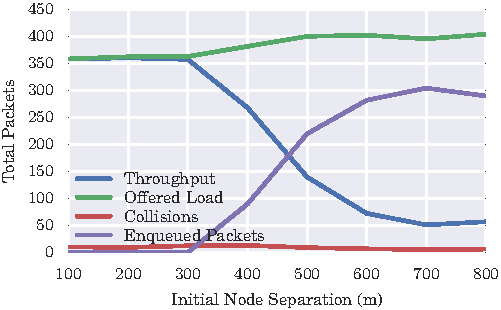
\includegraphics[width=\textwidth]{separation_throughput_performance_bella_all_mobile}
    \caption{Packet delivery}
    \label{fig:separation_throughput_performance_bella_all_mobile}
  \end{subfigure}
  %
  \begin{subfigure}[t]{0.5\textwidth}
    \centering
    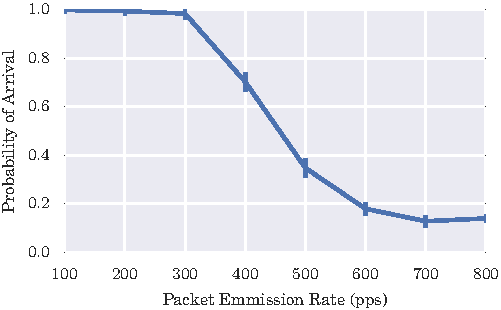
\includegraphics[width=\textwidth]{separation_prod_breakdown_bella_all_mobile}
    \caption{Probability of arrival}
    \label{fig:separation_prod_breakdown_bella_all_mobile}
  \end{subfigure}

  \begin{subfigure}[t]{0.5\textwidth}
    \centering
    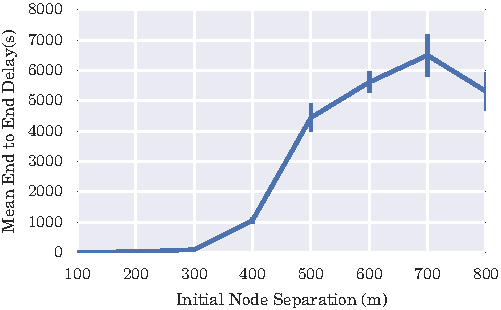
\includegraphics[width=\textwidth]{separation_delay_variation_bella_all_mobile}
    \caption{End-to-end delay}
    \label{fig:separation_delay_variation_bella_all_mobile}
  \end{subfigure}
  %
  \begin{subfigure}[t]{0.5\textwidth}
    \centering
    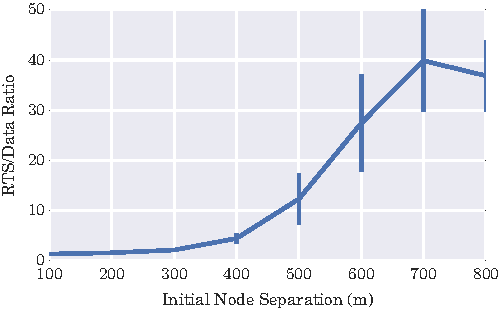
\includegraphics[width=\textwidth]{separation_rts_ratio_bella_all_mobile}
    \caption{RTS Ratios}
    \label{fig:separation_rts_ratio_bella_all_mobile}
  \end{subfigure}
  \caption{Network performance varying node separation for the all mobile case}
  \label{fig:separation_bella_all_mobile}
\end{figure}


\begin{figure}[tp!]
  \begin{subfigure}[t]{0.5\textwidth}
    \centering
    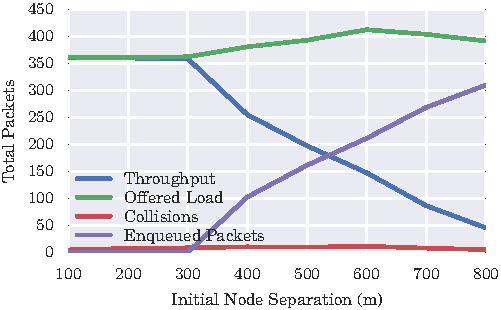
\includegraphics[width=\textwidth]{separation_throughput_performance_bella_allbut1_mobile}
    \caption{Packet delivery}
    \label{fig:separation_throughput_performance_bella_allbut1_mobile}
  \end{subfigure}
  %
  \begin{subfigure}[t]{0.5\textwidth}
    \centering
    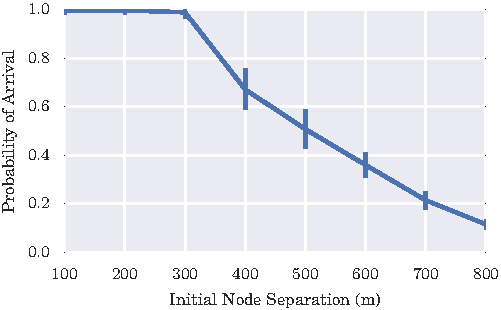
\includegraphics[width=\textwidth]{separation_prod_breakdown_bella_allbut1_mobile}
    \caption{Probability of arrival}
    \label{fig:separation_prod_breakdown_bella_allbut1_mobile}
  \end{subfigure}

  \begin{subfigure}[t]{0.5\textwidth}
    \centering
    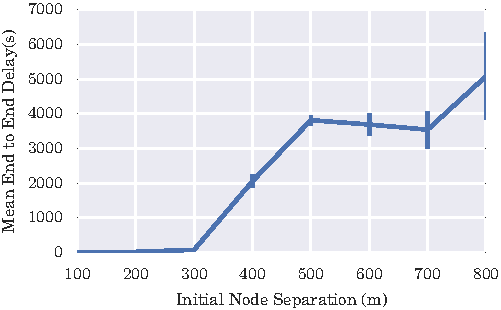
\includegraphics[width=\textwidth]{separation_delay_variation_bella_allbut1_mobile}
    \caption{End-to-end delay}
    \label{fig:separation_delay_variation_bella_allbut1_mobile}
  \end{subfigure}
  %
  \begin{subfigure}[t]{0.5\textwidth}
    \centering
    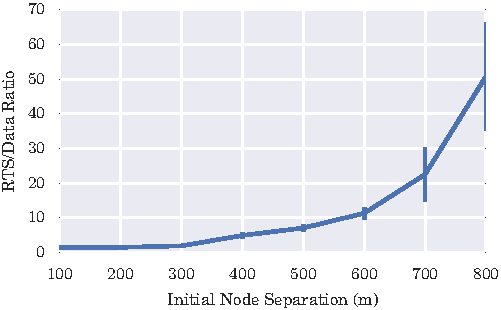
\includegraphics[width=\textwidth]{separation_rts_ratio_bella_allbut1_mobile}
    \caption{RTS Ratios}
    \label{fig:separation_rts_ratio_bella_allbut1_mobile}
  \end{subfigure}
  \caption{Network performance varying node separation for the all-but-one mobile case}
  \label{fig:separation_bella_allbut1_mobile}
\end{figure}

\begin{figure}[bp!]
  \begin{subfigure}[t]{0.5\textwidth}
    \centering
    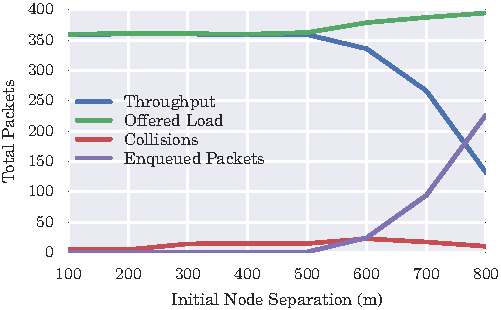
\includegraphics[width=\textwidth]{separation_throughput_performance_bella_single_mobile}
    \caption{Packet delivery}
    \label{fig:separation_throughput_performance_bella_single_mobile}
  \end{subfigure}
  %
  \begin{subfigure}[t]{0.5\textwidth}
    \centering
    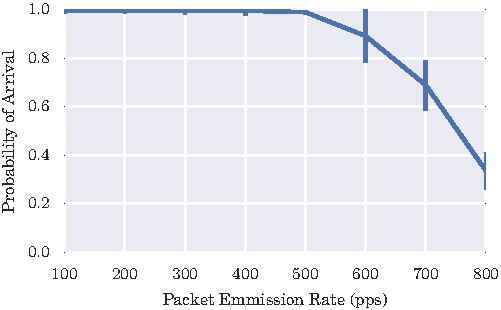
\includegraphics[width=\textwidth]{separation_prod_breakdown_bella_single_mobile}
    \caption{Probability of arrival}
    \label{fig:separation_prod_breakdown_bella_single_mobile}
  \end{subfigure}

  \begin{subfigure}[t]{0.5\textwidth}
    \centering
    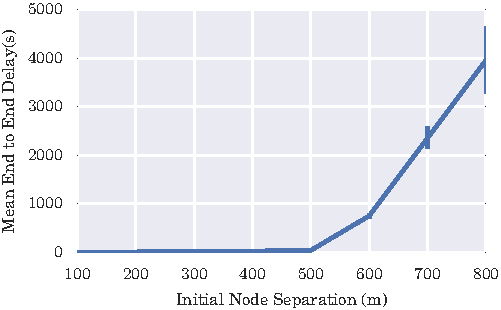
\includegraphics[width=\textwidth]{separation_delay_variation_bella_single_mobile}
    \caption{End-to-end delay}
    \label{fig:separation_delay_variation_bella_single_mobile}
  \end{subfigure}
  %
  \begin{subfigure}[t]{0.5\textwidth}
    \centering
    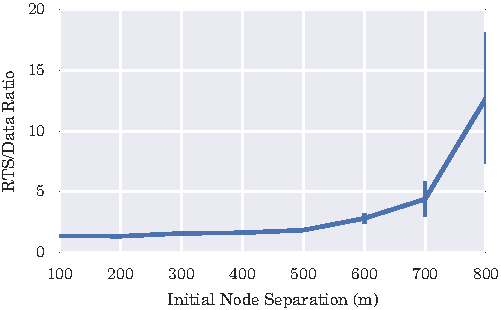
\includegraphics[width=\textwidth]{separation_rts_ratio_bella_single_mobile}
    \caption{RTS Ratios}
    \label{fig:separation_rts_ratio_bella_single_mobile}
  \end{subfigure}
  \caption{Network performance varying node separation for the single mobile case}
  \label{fig:separation_bella_single_mobile}
\end{figure}


\clearpage

\section{Combined Scale Factor Analysis}

Its clear from the previous results that the relationship between emission rates, separations and mobilities is tightly coupled and not totally clear cut. 
To arrive at a more optimal operating region, a coupled analysis is performed across both emission rate and initial separation distance.

Given what has been discussed so far; it's clear that in identifying an appropriate operating region, it is important to not only ensure throughput, but that that throughput is timely.
For instance, in~\autoref{fig:separation_bella_single_mobile} (tabulated in~\autoref{tab:separation_bella_single_mobile}), a small increase in separation beyond the apparent throughput-peak at 500$m$ to 600$m$, which constitutes an increased ideal marine acoustic ``time of flight'' between nodes by 0.02$s$, increases the average actual delay by 1800\%. 

To capture these performance requirements, the feature scaled product of Throughput and Delay is taken and plotted against rate and separation in~\autoref{fig:2d_normed_product}.\todo[inline]{This does NOT make for easy comparison between graphs as the scaling is different for each mobility, but I need to think about how to fairly solve this}



\begin{figure}[h]
  \begin{subfigure}[t]{0.5\textwidth}
    \centering
    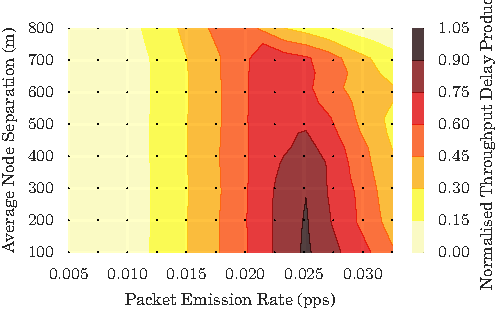
\includegraphics[width=\textwidth]{2d_normed_product_bella_static}
    \caption{Static}
    \label{fig:2d_normed_product_bella_static}
  \end{subfigure}
  \begin{subfigure}[t]{0.5\textwidth}
    \centering
    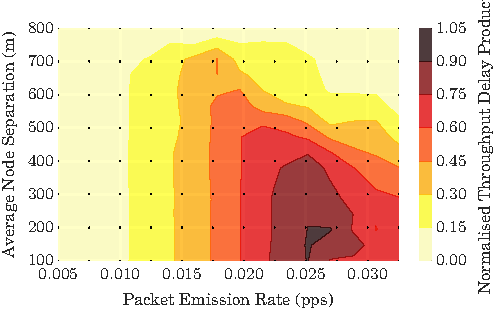
\includegraphics[width=\textwidth]{2d_normed_product_bella_single_mobile}
    \caption{Single Mobile}
    \label{fig:2d_normed_product_bella_single_mobile}
  \end{subfigure}
  
  \begin{subfigure}[t]{0.5\textwidth}
    \centering
    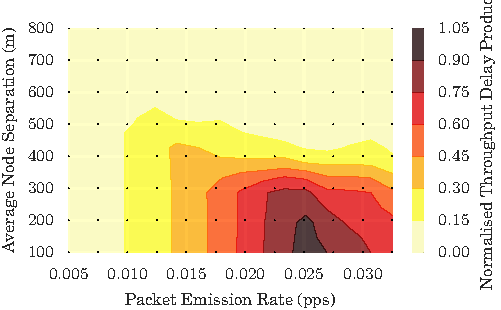
\includegraphics[width=\textwidth]{2d_normed_product_bella_allbut1_mobile}
    \caption{All-but-one Mobile}
    \label{fig:2d_normed_product_bella_allbut1_mobile}
  \end{subfigure}
  \begin{subfigure}[t]{0.5\textwidth}
    \centering
    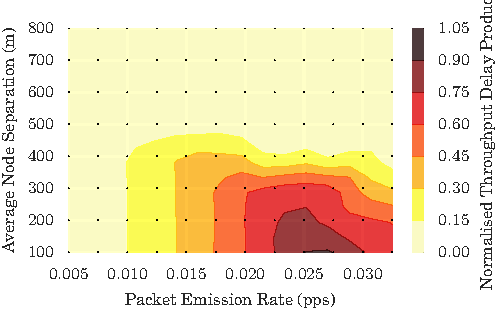
\includegraphics[width=\textwidth]{2d_normed_product_bella_all_mobile}
    \caption{All Mobile}
    \label{fig:2d_normed_product_bella_all_mobile}
  \end{subfigure}
  \caption{Normalised Throughput-Delay Product for all mobilities under varying separation and emission rate}
  \label{fig:2d_normed_product}
\end{figure}


\begin{table}[h]
	\caption{Tabular view of data from~\autoref{fig:separation_bella_single_mobile}, including ideal propagation time} \label{tab:separation_bella_single_mobile}
	\begin{center}
		\hyphenpenalty 100000
    \begin{tabular}{
            *{2}{@{\hspace{1em}}r@{\hspace{1em}}}
            *{3}{@{\hspace{1em}}p{0.1\textwidth} @{\hspace{1em}}}  }
\toprule
 Initial Node Separation (m) &  Delay(s) &  Probability of Arrival &  RTS/Data Ratio &  Ideal Delivery Time(s) \\
\midrule
                         100 &   10.3551 &                  0.9977 &          1.3546 &                  1.0314 \\
                         200 &   11.1631 &                  0.9973 &          1.3322 &                  1.1029 \\
                         300 &   24.2225 &                  0.9983 &          1.5650 &                  1.1743 \\
                         400 &   29.4864 &                  0.9965 &          1.6210 &                  1.2457 \\
                         500 &   41.7093 &                  0.9904 &          1.8331 &                  1.3171 \\
                         600 &  753.4040 &                  0.8922 &          2.8038 &                  1.3886 \\
                         700 & 2360.0826 &                  0.6899 &          4.3889 &                  1.4600 \\
                         800 & 3963.9830 &                  0.3360 &         12.7323 &                  1.5314 \\
\bottomrule
\end{tabular}

	\end{center}
\end{table}


\section{Conclusions}

An appropriate safe operating zone for marine communications has been established by investigating the impact of variations of the communications rate and physical distribution across the mobility scenarios.

These findings can be summaries as that when the separation is increased, the emission rate at which the network becomes saturated decreases, reducing overall throughput. 
This throughput degradation is tightly coupled with the mobility, as increasing mobility leads to increasing delays as routes are constantly broken, re-advertised and re-established. 
For instance, where all nodes are static, significant drops in throughput are not seen until node separation approaches 800m, nearly double the initial estimate. 
However, when all nodes are randomly walking the saturation point collapses from $0.025pps$ at $300m$ to $0.015pps$ at $400m$.\todo[inline]{Double Check These Numbers Before Release}
Our results indicate that the best area to continue operating in for a range of node separations is at $0.015pps$, and that a reasonable position scaling is from $100m$ to $300m$, beyond which communication becomes increasingly unstable, especially in terms of end-to-end delay.
These results are similar to work performed in \cite{Miquel2008}, and are expected in such a sparse, noisy, and contentious environment. 



The results from \autoref{fig:something} and \autoref{fig:somethingelse} show that the single-node mobility models don't capture the reality of the network \todo{this is a place holder for actual information}
The reason for this is that in other mobility combinations, the node targeted for misbehaviour ($n_1$) will already be behaving differently compared to the rest of the network regardless of the misbehaviour.
\todo{expand this section to include discussion and results of single mobility models}

%%%%%%%%%%%%%%%%%%%%%%%%%%%%%%%%%%%%%%%%%%%%%%%%%%%%%%%%%%%%%%%%%%%%%%%%%%%%%%%
